\subsection{Implementation}
\subsubsection{Step 1 - Database design}
Database design was done in design section above. From there, we are implementing concepts bellow.

\subsubsection{Step 2 - Create Docker containers}
\subsubsubsection{Docker compose for nodes/replica sets}

\begin{lstlisting}[caption=Docker Compose Nodes Version]
version: '2'
services:
\end{lstlisting}

\begin{lstlisting}[caption=Docker Compose Nodes for replica set 1]
mongo_ReplicaSet1_Node1:
    container_name: mongo_ReplicaSet1_Node1
    image: mongo
    command: mongod --shardsvr --replSet mongo_ReplicaSet1 --dbpath /data/db --port 27017
    ports:
      - 40117:27017
    expose:
      - "27017"
    environment:
      TERM: xterm
    volumes:
      - mongo_ReplicaSet1_Node1:/data/db
  mongo_ReplicaSet1_Node2:
    container_name: mongo_ReplicaSet1_Node2
    image: mongo
    command: mongod --shardsvr --replSet mongo_ReplicaSet1 --dbpath /data/db --port 27017
    ports:
      - 40127:27017
    expose:
      - "27017"
    environment:
      TERM: xterm
    volumes:
      - mongo_ReplicaSet1_Node2:/data/db
  mongo_ReplicaSet1_Node3:
    container_name: mongo_ReplicaSet1_Node3
    image: mongo
    command: mongod --shardsvr --replSet mongo_ReplicaSet1 --dbpath /data/db --port 27017
    ports:
      - 40137:27017
    expose:
      - "27017"
    environment:
      TERM: xterm
    volumes:
      - mongo_ReplicaSet1_Node3:/data/db
  mongo_ReplicaSet1_Arbiter:
    container_name: mongo_ReplicaSet1_Arbiter
    image: mongo
    command: mongod --shardsvr --replSet mongo_ReplicaSet1 --dbpath /data/db --port 27017
    ports:
      - 40138:27017
    expose:
      - "27017"
    environment:
      TERM: xterm
    volumes:
      - mongo_ReplicaSet1_Arbiter:/data/db
  mongo_ReplicaSet1_Backup:
    container_name: mongo_ReplicaSet1_Backup
    image: mongo
    command: mongod --shardsvr --replSet mongo_ReplicaSet1 --dbpath /data/db --port 27017
    ports:
      - 40139:27017
    expose:
      - "27017"
    environment:
      TERM: xterm
    volumes:
      - mongo_ReplicaSet1_Backup:/data/db
\end{lstlisting}

\begin{lstlisting}[caption=Docker Compose Nodes for replica set 2]
mongo_ReplicaSet2_Node1:
    container_name: mongo_ReplicaSet2_Node1
    image: mongo
    command: mongod --shardsvr --replSet mongo_ReplicaSet2 --dbpath /data/db --port 27017
    ports:
      - 40217:27017
    expose:
      - "27017"
    environment:
      TERM: xterm
    volumes:
      - mongo_ReplicaSet2_Node1:/data/db
  mongo_ReplicaSet2_Node2:
    container_name: mongo_ReplicaSet2_Node2
    image: mongo
    command: mongod --shardsvr --replSet mongo_ReplicaSet2 --dbpath /data/db --port 27017
    ports:
      - 40227:27017
    expose:
      - "27017"
    environment:
      TERM: xterm
    volumes:
      - mongo_ReplicaSet2_Node2:/data/db
  mongo_ReplicaSet2_Node3:
    container_name: mongo_ReplicaSet2_Node3
    image: mongo
    command: mongod --shardsvr --replSet mongo_ReplicaSet2 --dbpath /data/db --port 27017
    ports:
      - 40237:27017
    expose:
      - "27017"
    environment:
      TERM: xterm
    volumes:
      - mongo_ReplicaSet2_Node3:/data/db
  mongo_ReplicaSet2_Arbiter:
    container_name: mongo_ReplicaSet2_Arbiter
    image: mongo
    command: mongod --shardsvr --replSet mongo_ReplicaSet2 --dbpath /data/db --port 27017
    ports:
      - 40238:27017
    expose:
      - "27017"
    environment:
      TERM: xterm
    volumes:
      - mongo_ReplicaSet2_Arbiter:/data/db
  mongo_ReplicaSet2_Backup:
    container_name: mongo_ReplicaSet2_Backup
    image: mongo
    command: mongod --shardsvr --replSet mongo_ReplicaSet2 --dbpath /data/db --port 27017
    ports:
      - 40239:27017
    expose:
      - "27017"
    environment:
      TERM: xterm
    volumes:
      - mongo_ReplicaSet2_Backup:/data/db
\end{lstlisting}

\begin{lstlisting}[caption=Docker Compose Nodes for replica set 3]
mongo_ReplicaSet3_Node1:
    container_name: mongo_ReplicaSet3_Node1
    image: mongo
    command: mongod --shardsvr --replSet mongo_ReplicaSet3 --dbpath /data/db --port 27017
    ports:
      - 40317:27017
    expose:
      - "27017"
    environment:
      TERM: xterm
    volumes:
      - mongo_ReplicaSet3_Node1:/data/db
  mongo_ReplicaSet3_Node2:
    container_name: mongo_ReplicaSet3_Node2
    image: mongo
    command: mongod --shardsvr --replSet mongo_ReplicaSet3 --dbpath /data/db --port 27017
    ports:
      - 40327:27017
    expose:
      - "27017"
    environment:
      TERM: xterm
    volumes:
      - mongo_ReplicaSet3_Node2:/data/db
  mongo_ReplicaSet3_Node3:
    container_name: mongo_ReplicaSet3_Node3
    image: mongo
    command: mongod --shardsvr --replSet mongo_ReplicaSet3 --dbpath /data/db --port 27017
    ports:
      - 40337:27017
    expose:
      - "27017"
    environment:
      TERM: xterm
    volumes:
      - mongo_ReplicaSet3_Node3:/data/db
  mongo_ReplicaSet3_Arbiter:
    container_name: mongo_ReplicaSet3_Arbiter
    image: mongo
    command: mongod --shardsvr --replSet mongo_ReplicaSet3 --dbpath /data/db --port 27017
    ports:
      - 40338:27017
    expose:
      - "27017"
    environment:
      TERM: xterm
    volumes:
      - mongo_ReplicaSet3_Arbiter:/data/db
  mongo_ReplicaSet3_Backup:
    container_name: mongo_ReplicaSet3_Backup
    image: mongo
    command: mongod --shardsvr --replSet mongo_ReplicaSet3 --dbpath /data/db --port 27017
    ports:
      - 40339:27017
    expose:
      - "27017"
    environment:
      TERM: xterm
    volumes:
      - mongo_ReplicaSet3_Backup:/data/db
\end{lstlisting}

\begin{lstlisting}[caption=Docker Compose storage for nodes]
volumes:
  mongo_ReplicaSet1_Node1: {}
  mongo_ReplicaSet1_Node2: {}
  mongo_ReplicaSet1_Node3: {}
  mongo_ReplicaSet1_Arbiter: {}
  mongo_ReplicaSet1_Backup: {}
  mongo_ReplicaSet2_Node1: {}
  mongo_ReplicaSet2_Node2: {}
  mongo_ReplicaSet2_Node3: {}
  mongo_ReplicaSet2_Arbiter: {}
  mongo_ReplicaSet2_Backup: {}
  mongo_ReplicaSet3_Node1: {}
  mongo_ReplicaSet3_Node2: {}
  mongo_ReplicaSet3_Node3: {}
  mongo_ReplicaSet3_Arbiter: {}
  mongo_ReplicaSet3_Backup: {}
\end{lstlisting}
\subsubsubsection{Docker compose for config servers}
\begin{lstlisting}[caption=Docker Compose Config Version]
version: '2'
services:
\end{lstlisting}

\begin{lstlisting}[caption=Docker Compose Config 1]
mongo_Config1:
      container_name: mongo_Config1
      image: mongo
      command: mongod --configsvr --replSet mongo_ReplicaSet1_Conf --dbpath /data/db --port 27017
      environment:
        TERM: xterm
      expose:
        - "27017"
      volumes:
        - mongo_Config1:/data/db
\end{lstlisting}

\begin{lstlisting}[caption=Docker Compose Config 2]
mongo_Config2:
      container_name: mongo_Config2
      image: mongo
      command: mongod --configsvr --replSet mongo_ReplicaSet1_Conf --dbpath /data/db --port 27017
      environment:
        TERM: xterm
      expose:
        - "27017"
      volumes:
        - mongo_Config2:/data/db
\end{lstlisting}

\begin{lstlisting}[caption=Docker Compose Config 3]
  mongo_Config3:
      container_name: mongo_Config3
      image: mongo
      command: mongod --configsvr --replSet mongo_ReplicaSet1_Conf --dbpath /data/db --port 27017
      environment:
        TERM: xterm
      expose:
        - "27017"
      volumes:
        - mongo_Config3:/data/db
\end{lstlisting}

\begin{lstlisting}[caption=Docker Compose storage for Config]
volumes:
  mongo_Config1: {}
  mongo_Config2: {}
  mongo_Config3: {}
\end{lstlisting}
\subsubsubsection{Docker compose for routers}
\begin{lstlisting}[caption=Docker Compose Router Version]
version: '2'
services:
\end{lstlisting}

\begin{lstlisting}[caption=Docker Compose router 1]
mongo_Shard1:
    container_name: mongo_Shard1
    image: mongo
    command: mongos --configdb mongo_ReplicaSet1_Conf/mongo_Config1:27017,mongo_Config2:27017,mongo_Config3:27017 --port 27017 --bind_ip 0.0.0.0
    ports:
      - 27019:27017
    expose:
      - "27017"
    volumes:
      - /etc/localtime:/etc/localtime:ro
\end{lstlisting}

\begin{lstlisting}[caption=Docker Compose router 2]
  mongo_Shard2:
    container_name: mongo_Shard2
    image: mongo
    command: mongos --configdb mongo_ReplicaSet1_Conf/mongo_Config1:27017,mongo_Config2:27017,mongo_Config3:27017 --port 27017 --bind_ip 0.0.0.0
    ports:
      - 27020:27017
    expose:
      - "27017"
    volumes:
      - /etc/localtime:/etc/localtime:ro
\end{lstlisting}

\begin{lstlisting}[caption=Docker Compose router 3]
  mongo_Shard3:
    container_name: mongo_Shard3
    image: mongo
    command: mongos --configdb mongo_ReplicaSet1_Conf/mongo_Config1:27017,mongo_Config2:27017,mongo_Config3:27017 --port 27017 --bind_ip 0.0.0.0
    ports:
      - 27021:27017
    expose:
      - "27017"
    volumes:
      - /etc/localtime:/etc/localtime:ro
\end{lstlisting}
\subsubsubsection{Execute docker compose}
\paragraph{Run docker compose files}\mbox{}\\
setup replica $\xrightarrow{}$ set nodes - 5 nodes per 3 replica sets $\xrightarrow{}$ 15 docker nodes are created
\begin{lstlisting}[language=Bash, caption=Create 15 Mongo nodes]
sudo docker-compose -f docker-compose.yaml up -d
\end{lstlisting}
setup config $\xrightarrow{}$ 3 config (docker) servers are running
\begin{lstlisting}[language=Bash, caption=Create config servers]
sudo docker-compose -f mongod.yaml up -d
\end{lstlisting}
setup router $\xrightarrow{}$ 3 mongos (router) dockers are running
\begin{lstlisting}[language=Bash, caption=Create router servers]
sudo docker-compose -f mongos.yaml up -d
\end{lstlisting}

%=========================================================================================================
% configure config servers replica set
%=========================================================================================================
\paragraph{Configure config servers replica set}\mbox{}\\
Replica set 1
\begin{lstlisting}[language=Bash, caption=Set config1]
docker exec -it mongo_Config1 bash -c "echo 'rs.initiate(
    {_id: \"mongo_ReplicaSet1_Conf\",configsvr: true, members: [
        { _id : 0, host : \"mongo_Config1\" },
        { _id : 1, host : \"mongo_Config2\" }, 
        { _id : 2, host : \"mongo_Config3\" }
        ]
    })
' | mongosh"
\end{lstlisting}
Replica set 2
\begin{lstlisting}[language=Bash, caption=Set config2]
docker exec -it mongo_Config2 bash -c "echo 'rs.initiate(
    {_id: \"mongo_ReplicaSet1_Conf\",configsvr: true, members: [
        { _id : 0, host : \"mongo_Config1\" },
        { _id : 1, host : \"mongo_Config2\" }, 
        { _id : 2, host : \"mongo_Config3\" }
        ]
    }
)' | mongosh"
\end{lstlisting}
Replica set 3
\begin{lstlisting}[language=Bash, caption=Set config3]
docker exec -it mongo_Config3 bash -c "echo 'rs.initiate(
    {_id: \"mongo_ReplicaSet1_Conf\",configsvr: true, members: [
        { _id : 0, host : \"mongo_Config1\" },
        { _id : 1, host : \"mongo_Config2\" }, 
        { _id : 2, host : \"mongo_Config3\" }
        ]
    }
)' | mongosh"
\end{lstlisting}

%=========================================================================================================
% check config server replica set status
%=========================================================================================================
\paragraph{Check config server replica set status}\mbox{}\\
\begin{lstlisting}[language=Bash, caption=Check replica set status]
docker exec -it mongo_Config1 bash -c "echo 'rs.status()' | mongosh"
\end{lstlisting}

%=========================================================================================================
% build shard replica set
%=========================================================================================================
\paragraph{Build shard replica set}\mbox{}\\
Replica set 1
\begin{lstlisting}[language=Bash, caption=Build replica set 1]
docker exec -it mongo_ReplicaSet1_Node1 bash -c "echo 'rs.initiate(
    {_id : \"mongo_ReplicaSet1\", members: [
        { _id : 0, host : \"mongo_ReplicaSet1_Node1\" },
        { _id : 1, host : \"mongo_ReplicaSet1_Node2\" },
        { _id : 2, host : \"mongo_ReplicaSet1_Node3\" },
        { _id : 3, host : \"mongo_ReplicaSet1_Arbiter\", arbiterOnly: true},
        { _id : 4, host : \"mongo_ReplicaSet1_Backup\", hidden: true}
        ]
    }
)' | mongosh"
\end{lstlisting}
Replica set 2
\begin{lstlisting}[language=Bash, caption=Build replica set 2]
docker exec -it mongo_ReplicaSet2_Node1 bash -c "echo 'rs.initiate(
    {_id : \"mongo_ReplicaSet2\", members: [
        { _id : 0, host : \"mongo_ReplicaSet2_Node1\" },
        { _id : 1, host : \"mongo_ReplicaSet2_Node2\" },
        { _id : 2, host : \"mongo_ReplicaSet2_Node3\" },
        { _id : 3, host : \"mongo_ReplicaSet2_Arbiter\", arbiterOnly: true},
        { _id : 4, host : \"mongo_ReplicaSet2_Backup\", hidden: true}
        ]
    }
)' | mongosh"
\end{lstlisting}
Replica set 3
\begin{lstlisting}[language=Bash, caption=Build replica set 3]
docker exec -it mongo_ReplicaSet3_Node1 bash -c "echo 'rs.initiate(
    {_id : \"mongo_ReplicaSet3\", members: [
        { _id : 0, host : \"mongo_ReplicaSet3_Node1\" },
        { _id : 1, host : \"mongo_ReplicaSet3_Node2\" },
        { _id : 2, host : \"mongo_ReplicaSet3_Node3\" },
        { _id : 3, host : \"mongo_ReplicaSet3_Arbiter\", arbiterOnly: true},
        { _id : 4, host : \"mongo_ReplicaSet3_Backup\", hidden: true}
        ]
    }
)' | mongosh"
\end{lstlisting}

%=========================================================================================================
% check status primary-secondary
%=========================================================================================================
\paragraph{Check status primary-secondary}\mbox{}\\
Status for replica set 1
\begin{lstlisting}[language=Bash, caption=Check status of replica set 1]
docker exec -it mongo_ReplicaSet1_Node1 bash -c "echo 'rs.status()' | mongosh"
\end{lstlisting}
Status for replica set 2
\begin{lstlisting}[language=Bash, caption=Check status of replica set 2]
docker exec -it mongo_ReplicaSet2_Node1 bash -c "echo 'rs.status()' | mongosh"
\end{lstlisting}
Status for replica set 3
\begin{lstlisting}[language=Bash, caption=Check status of replica set 3]
docker exec -it mongo_ReplicaSet3_Node1 bash -c "echo 'rs.status()' | mongosh"
\end{lstlisting}

%=========================================================================================================
% introduce shard to the routers
%=========================================================================================================
\paragraph{Introduce replica set to the routers}\mbox{}\\
Add mongo{\_}Shard1
\begin{lstlisting}[language=Bash, caption=Introduce replica 1]
docker exec -it mongo_Shard1 bash -c "echo 'sh.addShard(\"mongo_ReplicaSet1/mongo_ReplicaSet1_Node1\")' | mongosh"
\end{lstlisting}
Add mongo{\_}Shard2
\begin{lstlisting}[language=Bash, caption=Introduce replica 2]
docker exec -it mongo_Shard2 bash -c "echo 'sh.addShard(\"mongo_ReplicaSet2/mongo_ReplicaSet2_Node1\")' | mongosh"
\end{lstlisting}
Add mongo{\_}Shard3
\begin{lstlisting}[language=Bash, caption=Introduce replica 3]
docker exec -it mongo_Shard3 bash -c "echo 'sh.addShard(\"mongo_ReplicaSet3/mongo_ReplicaSet3_Node1\")' | mongosh"
\end{lstlisting}

%=========================================================================================================
% get shard status
%=========================================================================================================
\paragraph{Get shard status}\mbox{}\\
\begin{lstlisting}[language=Bash, caption=Get shard status]
docker exec -it mongo_Shard1 bash -c "echo 'sh.status()' | mongosh"
\end{lstlisting}

%=========================================================================================================
% create test db
%=========================================================================================================
\paragraph{Create test db}\mbox{}\\
Create test db in shard mongo{\_}ReplicaSet{\_}1 for testing.
\begin{lstlisting}[language=Bash, caption=Create test db]
docker exec -it mongo_ReplicaSet1_Node1 bash -c "echo 'use testDb' | mongosh"
\end{lstlisting}

%=========================================================================================================
% enable sharding for new db
%=========================================================================================================
\paragraph{Enable sharding for new db}\mbox{}\\
Test sharding of new database.
\begin{lstlisting}[language=Bash, caption=Enable sharding for new db]
docker exec -it mongo_Shard1 bash -c "echo 'sh.enableSharding(\"testDb\")' | mongosh"
\end{lstlisting}

%=========================================================================================================
% create test collection
%=========================================================================================================
\paragraph{Create test collection}\mbox{}\\
Create test collection for further testing.
\begin{lstlisting}[language=Bash, caption=Create test collection RS1]
docker exec -it mongo_ReplicaSet1_Node1 bash -c "echo 'db.createCollection(\"testDb.testCollection\")' | mongosh"
\end{lstlisting}
\begin{lstlisting}[language=Bash, caption=Create test collection RS2]
docker exec -it mongo_ReplicaSet2_Node1 bash -c "echo 'db.createCollection(\"testDb.testCollection\")' | mongosh"
\end{lstlisting}
\begin{lstlisting}[language=Bash, caption=Create test collection RS3]
docker exec -it mongo_ReplicaSet3_Node1 bash -c "echo 'db.createCollection(\"testDb.testCollection\")' | mongosh"
\end{lstlisting}

%=========================================================================================================
% shard based on the key
%=========================================================================================================
\paragraph{Shard based on the key}\mbox{}\\
Test sharding collection based on the key.
\begin{lstlisting}[language=Bash, caption=Shard based on the key]
docker exec -it mongo_Shard1 bash -c "echo 'sh.shardCollection(\"testDb.testCollection\", {\"shardingField\" : 1})' | mongosh"
\end{lstlisting}
\subsubsubsection{Showcase of docker containers}
At the end we have 21 docker containers that are database related. All of the Docker containers are on local network (localhost) in our case. In the table bellow, we can see the function they have.

\begin{center}
\begin{longtable}{ |m{5.5cm}|m{6cm}|m{1.5cm}| } 
 \hline
    Container name & Container description & Port \\ 
 \hline
 \hline
    mongo{\_}ReplicaSet1{\_}Node1 & Storage node 1 for replica set 1 & 40117\\ 
 \hline
    mongo{\_}ReplicaSet1{\_}Node2 & Storage node 2 for replica set 1 & 40127\\ 
 \hline
    mongo{\_}ReplicaSet1{\_}Node3 & Storage node 3 for replica set 1 & 40137\\ 
 \hline
    mongo{\_}ReplicaSet1{\_}Arbiter & Tie breaker for replica set 1 & 40147\\ 
 \hline
    mongo{\_}ReplicaSet1{\_}Backup & Backup node for replica set 1 & 40157\\ 
 \hline
 \hline
    mongo{\_}ReplicaSet2{\_}Node1 & Storage node 1 for replica set 2 & 40217\\ 
 \hline
    mongo{\_}ReplicaSet2{\_}Node2 & Container 1 for replica set 2 & 40227\\ 
 \hline
    mongo{\_}ReplicaSet2{\_}Node3 & Container 1 for replica set 2 & 40237\\ 
 \hline
    mongo{\_}ReplicaSet2{\_}Arbiter & Tie breaker for replica set 2 & 40247\\ 
 \hline
    mongo{\_}ReplicaSet2{\_}Backup & Backup node for replica set 2 & 40257\\ 
 \hline
 \hline
    mongo{\_}ReplicaSet3{\_}Node1 & Storage node 1 for replica set 3 & 40317\\ 
 \hline
    mongo{\_}ReplicaSet3{\_}Node2 & Storage node 2 for replica set 3 & 40327\\ 
 \hline
    mongo{\_}ReplicaSet3{\_}Node3 & Storage node 3 for replica set 3 & 40337\\ 
 \hline
    mongo{\_}ReplicaSet3{\_}Arbiter & Tie breaker for replica set 3 & 40347\\ 
 \hline
    mongo{\_}ReplicaSet3{\_}Backup & Backup node for replica set 3 & 40357\\ 
 \hline
 \hline
    mongo{\_}Config1 & Configuration server 1 & 27017\\ 
 \hline
    mongo{\_}Config2 & Configuration server 2 & 27017\\ 
 \hline
    mongo{\_}Config3 & Configuration server 3 & 27017\\ 
 \hline
 \hline
    mongo{\_}Shard1 & Main router & 27019\\ 
 \hline
    mongo{\_}Shard2 & Backup router 1 & 27020\\ 
 \hline
    mongo{\_}Shard3 & Backup router 2 & 27021\\ 
 \hline
\caption{Containers used described}
\end{longtable}
\end{center}

\begin{figure}[H]
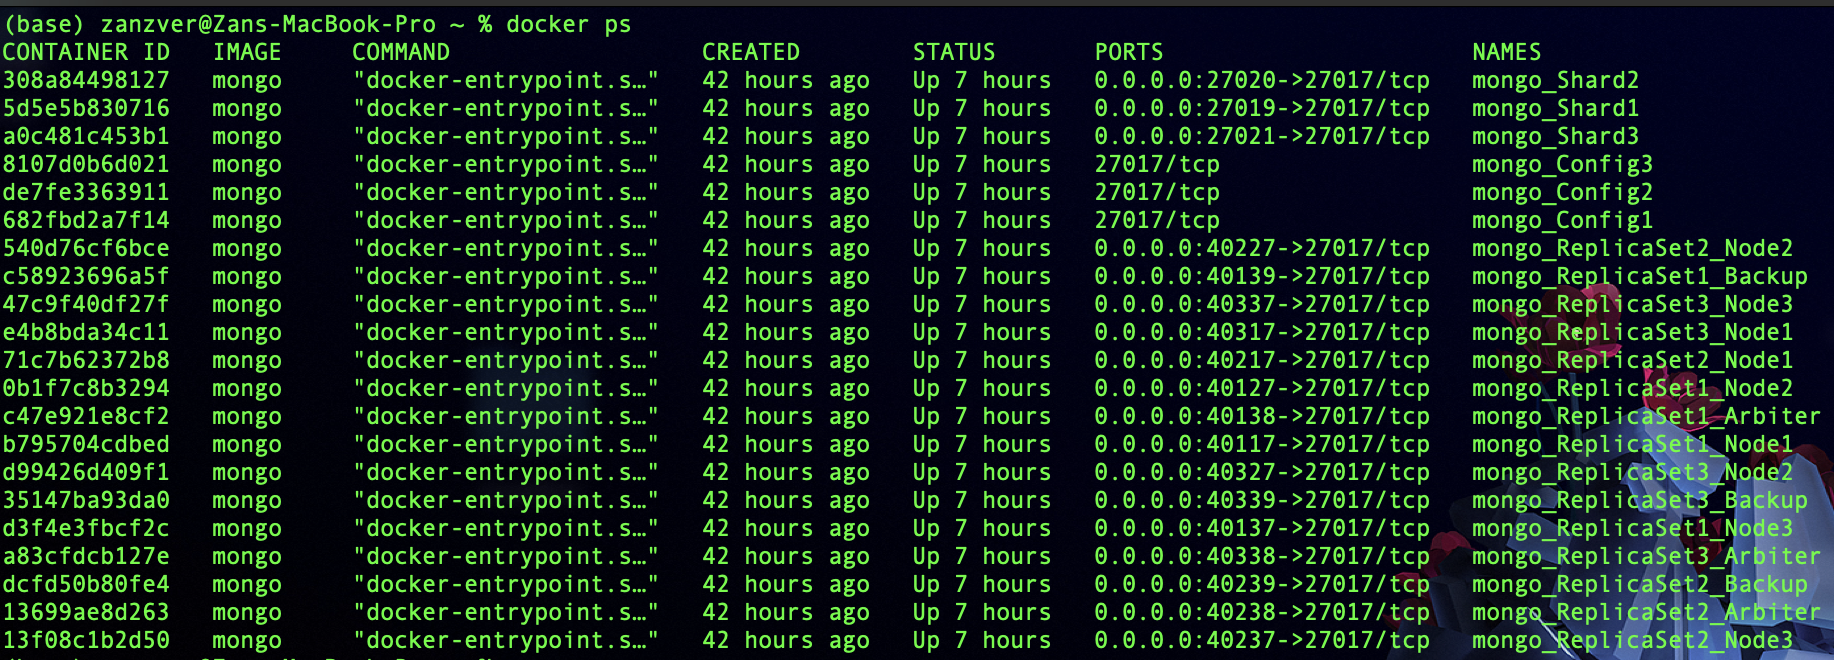
\includegraphics[scale=0.45]{img/allDockerContainers.png}
\centering
\caption{Containers displayed in terminal}
\end{figure}

\subsubsection{Step 3 - Fill the database}
To fill the database, Python scrip was used for inserting random data.
\newline
First thing is to specify how many users we want. 
\begin{lstlisting}[language=Python, caption=Call createUser function]
createUser(10)
\end{lstlisting}
Based on the input number (10 in our case) users are going to be created.
\begin{lstlisting}[language=Python, caption=Showcase of createUser function]
def createUser(num):
    for i in range(num):
        firstname = names.get_first_name()
        lastname = names.get_last_name()
        items = ["", str(random.randrange(1,999))]
        random_item = random.choice(items)
        random_email = random.choice(emailProviders)
        random_address = real_random_address()
        #print(random_item)
        mydict = {
                "Username": firstname + lastname,
                "Password": randomword(10),
                "Email": firstname + "." + lastname + random_item + random_email,
                "Name": firstname,
                "Surname": lastname,
                "Location": {
                    "Address": [
                        random_address["address1"],
                        random_address["address2"]
                    ],
                    "Postcode": random_address["postalCode"],
                    "City": random_address["state"],
                    "Country": "United States"
                }
        }
        x = colUsers.insert_one(mydict)
        createItAll(x.inserted_id)
        createHistory(x.inserted_id)
\end{lstlisting}
When we create the user, we also create devices for the user.
\begin{lstlisting}[language=Python, caption=Showcase of createItAll function]
def createItAll(UserID):
    myDict = createDevices()
    colIoT_Customer_Device.insert_one(
        { "UserID" : str(UserID),
          "smart_light": myDict["smart_light"],
          "smart_fridge": myDict["smart_fridge"],
          "smart_vacuum": myDict["smart_vacuum"]
        })
    
    dict1 = createDeviceInfo()
    try:
        dict2 = colIoT_Device_Info.find_one()
        for deviceTypes in dict1.keys():
            for manufacturer in dict1[deviceTypes].keys():
                for modelName in list(dict1[deviceTypes][manufacturer])[0].keys():
                    for serialNumber in list(dict2[deviceTypes][manufacturer])[0][modelName]["Serial_Numbers"]:
                        list(dict1[deviceTypes][manufacturer])[0][modelName]["Serial_Numbers"].append(serialNumber)
        
        oldquery = colIoT_Device_Info.find_one()
        newquery = { "$set": dict1 }
        
        colIoT_Device_Info.update_one(oldquery, newquery)
    except:
        colIoT_Device_Info.insert_one(dict1)
\end{lstlisting}
As noted in the code, history for device is also generated.
\begin{lstlisting}[language=Python, caption=Showcase of createHistory]
def createHistory(userID):
    lightHistoryGenerator = random.randrange(1,30)
    fridgeHistoryGenerator = random.randrange(1,30)
    vacuumHistoryGenerator = random.randrange(1,30)
    for i in range(lightHistoryGenerator):
        colIoT_Device_History.insert_one({str(userID): {"1": createTheSmartLight()["Device_Status"]}})
    
    for i in range(fridgeHistoryGenerator):
        colIoT_Device_History.insert_one({str(userID): {"2": createTheFridge()["Device_Status"]}})
        
    for i in range(vacuumHistoryGenerator):
        colIoT_Device_History.insert_one({str(userID): {"3": createTheVauum()["Device_Status"]}})
\end{lstlisting}

\subsubsection{Step 4 - API}
Connect the database with API
\begin{lstlisting}[language=JavaScript, caption=Showcase of Mongoose connection to database]
const mongoose = require("mongoose");

mongoose.connect('mongodb://localhost:27019,localhost:27020,localhost:27021/initialDB', {useNewUrlParser: true}, (err) => {
    if(!err){
        console.log("MongoDB Conncetion Succeeded!")
    }
    else{
        console.log("Error in DB connection: " + err)
    }
});

require("./employee.model");
require("./user.model.js");
require("./IoT_Customer_Device.model.js");
require("./IoT_Device_Info.model.js");
\end{lstlisting}

\subsubsubsection{Step 5 - Indexes}
To improve database performance, we have added indexes \parencite{web:MongoIndexes}. With this, database management system has a faster way to identify location of document in our collection. Listed bellow we can see collections and their indexes.
\begin{center}
\begin{longtable}{ |m{4cm}|m{9cm}| } 
 \hline
 Collections name & Index description \\ 
 \hline
  users &   
  \begin{itemize}
    \item Index type: regular
    \item This collection can benefit on stock index {\_}id. Any other index would not be benefitial at the moment since we are not using this collection a lot. Most of the queries are done by {\_}id.
  \end{itemize} \\
  
  \hline
  iot{\_}customer{\_}devices &  
  \begin{itemize}
    \item Index type: regular
    \item In this collection we have a custom index with the name of UserID. As name suggests, this field has the value from collection users with users ID. Comparison bellow shows that index did not save us much time but on the document examined section, we have navigated straight to our document. If this would be larger database, time would be much bigger concern.
    \item Performance without index
    \begin{itemize}
        \item executionTimeMillis : 2
        \item totalKeysExamined : 0
        \item totalDocsExamined : 1200
    \end{itemize}
    \item Performance with index
    \begin{itemize}
        \item executionTimeMillis : 3
        \item totalKeysExamined : 1
        \item totalDocsExamined : 1
    \end{itemize}
  \end{itemize} \\
  
  \hline
  iot{\_}device{\_}info &  
  \begin{itemize}
    \item Index type: regular
    \item This collection is small (at the moment) and it does not benefit much from indexing. But in case we wanted to index it, we would do it by device type and its manufacturer.
    \item Performance without index
    \begin{itemize}
        \item executionTimeMillis : 0
        \item totalKeysExamined : 0
        \item totalDocsExamined : 1
    \end{itemize}
    \item Performance with index
    \begin{itemize}
        \item executionTimeMillis : 0
        \item totalKeysExamined : 0
        \item totalDocsExamined : 1
    \end{itemize}
  \end{itemize} \\
  
  \hline
 iot{\_}device{\_}history &  
  \begin{itemize}
    \item Index type: regular
    \item History is build as UserID (key): DeviceID (value) and in the DeviceID we have history. The idea was to create a temporary index on UserID. So, when user logs in, index is created in database and when they log out, index is removed. Upon creating index, we have noticed that indexing seems to not be performing as well. In the future, we would break the UserID (key): DeviceID (value) to UserID: value of key and to DeviceID: value of device.
    \item Performance without index
    \begin{itemize}
        \item executionTimeMillis : 37
        \item totalKeysExamined : 0
        \item totalDocsExamined : 53838
    \end{itemize}
    \item Performance with index
    \begin{itemize}
        \item executionTimeMillis : 55
        \item totalKeysExamined : 53838
        \item totalDocsExamined : 53838
    \end{itemize}
  \end{itemize} \\
  \hline
\caption{Indexes on collections}
\end{longtable}
\end{center}

\begin{figure}[H]
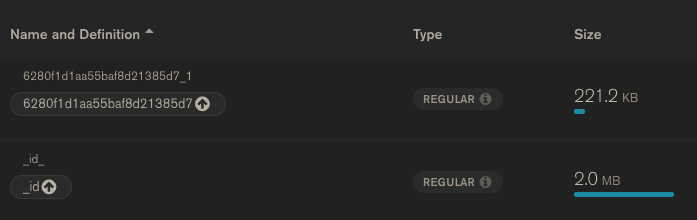
\includegraphics[scale=0.55]{img/iot_device_history-index.jpeg}
\centering
\caption{iot{\_}device{\_}history collection index}
\end{figure}


\begin{figure}[H]
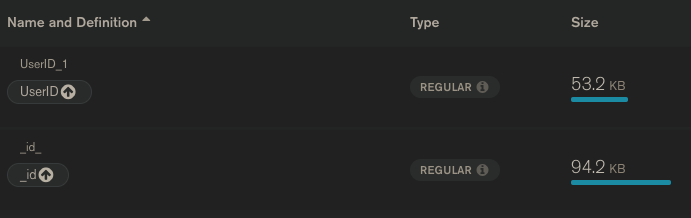
\includegraphics[scale=0.55]{img/iot_customer_devices-index.jpeg}
\centering
\caption{iot{\_}customer{\_}devices collection index}
\end{figure}


\begin{figure}[H]
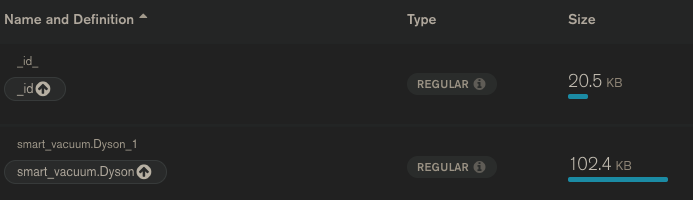
\includegraphics[scale=0.55]{img/iot_device_info-index.jpeg
}
\centering
\caption{iot{\_}device{\_}info collection index}
\end{figure}


\begin{figure}[H]
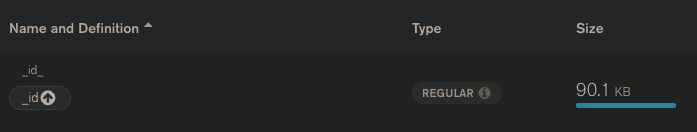
\includegraphics[scale=0.55]{img/users-index.jpeg}
\centering
\caption{users collection index}
\end{figure}
